\documentclass[12pt]{article}

\usepackage{graphicx,url}

\usepackage[brazilian]{babel}
\usepackage[utf8x]{inputenc}
\usepackage{amssymb,amsmath}
\usepackage[T1]{fontenc}
\usepackage{verbatim}
\usepackage{hyperref}
\usepackage{fullpage}
\usepackage{multicol}
\usepackage{lmodern}
\usepackage{xcolor}
\usepackage{listings}
\usepackage[colorinlistoftodos]{todonotes}
\usepackage{fixltx2e}
\usepackage{longtable}
\usepackage{float}
\usepackage{wrapfig}
\usepackage{soul}
\usepackage{textcomp}
\usepackage{marvosym}
\usepackage{wasysym}
\usepackage{latexsym}
\usepackage{amssymb}
\usepackage{hyperref}
\tolerance=1000
\usepackage{geometry}
\geometry{left=0.7in,right=0.7in,top=1in,bottom=1in}
\providecommand{\alert}[1]{\textbf{#1}}

\lstset{%
 basicstyle=\small\ttfamily\color{black!85},
 breaklines = true,
 keywordstyle=\bfseries\color{black},
 emphstyle=\color{blue},
 columns=fullflexible,
 showstringspaces=false
}%

\lstdefinelanguage{GODSmalltalk}
  {keywords={SSSpreadsheetData, SSSheet, SSRow, SSCell},
  morestring=[b]{'},
  stringstyle=\color{purple},
  alsoletter={:}, 
  emph={new}
}

% Python environment
\lstnewenvironment{godCode}[1][]
{
\lstset{language=GODSmalltalk,
    #1}
}
{}


\graphicspath { {figures/} }
\setlength{\parindent}{0cm}

\begin{document}

\section{GODAcademics '15}

\textbf{Grupo:}\textit{Pedro Bruel, António Martins Miranda, António Castro Júnior}

\textbf{Contato:}\{pedro.bruel, amartmiranda, to.junior.25\}@gmail.com\\

O GODAcademics é um agregador de informações acadêmicas. A partir de um perfil
do Google Scholar, ou de um currículo Lattes, esta aplicação constroi 
um relatório resumindo as informações obtidas de diversas fontes.

\subsection{Objetivos}

Os objetivos para o primeiro semestre de 2015 foram:

\begin{itemize}
    \item Refatoração de Testes;
    \item Aumentar a Cobertura de Testes;
    \item Aprimorar a página \emph{web} do projeto;
    \item Implementar a busca \emph{fuzzy} de texto (distância de Levenshtein e cálculo da similaridade);
    \item Implementar uma interface com o Sistema Lattes.
\end{itemize}

\subsection{Refatorações e Cobertura de Testes}

Adicionamos mais casos de teste para a busca por \emph{strings}
relativas a conferências e \emph{journals}. Separamos alguns testes
de unidade que agrupavam vários métodos no mesmo caso de teste.

\subsection{Página do Projeto}

Foi implementada uma nova interface para a página \emph{web}
do GODAcademics. A \emph{Issue} 450 no \emph{redmine} descreve
alguns pedidos de alterações feitos ao grupo \emph{GODWeb},
para que nossa implementação pudesse ser utilizada.

Habilitamos as visualizações para as buscas no \emph{Google Scholar}
e currículo \emph{Lattes}. A busca agora é feita através de um único
campo, e a distinção entre as fontes é feita baseando-se na assinatura
do \emph{link} submetido.

\subsection{Busca \emph{Fuzzy}}

Foi implementado um algoritmo para a busca aproximada de texto.
O algoritmo utilizado foi o cálculo da distância de \emph{Levenshtein},
que permite calcular distâncias entre \emph{strings} e fazer a busca
\emph{fuzzy}. Por exemplo, a busca por "\emph{plos comp bio}" deve retornar
resultados para o \emph{journal} \emph{PLOS Computational Biology}.

O método implementado foi \texttt{levenshteinDistanceBetween:and:},
que recebe duas \emph{strings} e calcula a distância entre elas.

Tivemos alguns problemas com a implementação dos testes para esse algoritmo,
pois o arcabouço de testes para \emph{Smalltalk} utilizado impõe limites
para a duração dos testes de unidade.

\subsection{Interface com o Sistema Lattes}

Tivemos problemas com o interfaceamento e obtenção de informações
de Currículos \emph{Lattes}, pois o \emph{site} adotou, recentemente,
um sistema de \emph{CAPTCHA}. Uma tentativa de contornar esse problema
foi utilizar o \emph{scriptLattes}, uma ferramenta para obtenção desses dados.
No entanto, a ferramenta também não funcionou por conta do \emph{CAPTCHA}.

Decidimos então implementar o \emph{parsing} de arquivos html correspondentes
a perfis do Currículo Lattes. Desta forma, quando for possível contornar as
restrições impostas pelo sistema, já teremos a estrutura para obtenção de 
informações sobre os pesquisadores pronta.

Criamos a classe \texttt{ACADInput}, que permite a criação de uma entrada
genérica para o \emph{GODAcademics}. Um objeto \texttt{ACADInput} armazena
a \emph{url} de um perfil do \emph{Google Scholar} ou Currículo \emph{Lattes},
e referencia um \emph{handler} que contém informações sobre as \emph{tags html}
correspondentes ao perfil.


\subsection{Trabalhos Futuros}

Seria interessante conseguir contornar o \emph{CAPTCHA} para o acesso ao
Currículo \emph{Lattes}. Uma ideia para isso seria repassar ao usuário a
tarefa de preenchê-lo, seja redirecionando à página do currículo e depois
retornando, ou lendo e mostrando o mesmo \emph{CAPTCHA} à partir do
GODAcademics. Uma vez que o \emph{parser} para o \emph{Lattes} já está
implementado, contornar o \emph{CAPTCHA} permitiria o acesso às informações
disponíveis no currículo.

Gostaríamos de implementar mecanismos de análise dos grupos de pesquisa
ao redor do Brasil, agrupando temas, laboratórios e pesquisadores 
geograficamente. Isso poderia ser feito através de informações disponíveis
nos Currículos \emph{Lattes} de pesquisadores.

Essas informações geográficas poderiam ser utilizadas na forma de um mapa
exibido pelo GOD, que mostraria a distribuição e o interesse em determinado
tema de pesquisa no Brasil.

Outra possibilidade poderia envolver a implementação de um \emph{webcrawler}
para o Sistema \emph{Lattes}, que agregasse informações continuamente sobre
os currículos.\\

Algumas correcções e otimimazões a serem levadas em conta:
\begin{itemize}
	\item na home do \emph{GODAcademics}, validar os campo para a inserção de links; 
	\item melhorar eficência  do atual algoritmo \emph{fuzzy} (cálcula da similaridade entre duas strings por meio da distância do  \emph{Levenshtein}) ou implementar outra estratégia de busca \emph{fuzzy} mais elaborada(algoritmos do Smith–Waterman, Needleman–Wunsch,Jaro–Winkler, etc);
	\item aumentar a precisão do \emph{Levenshtein}, fazendo um tratamento mais rigoroso das strings a serem comparadas ;
	\item estudar e determinar qual a melhor porcentagem de similaridade a ser usado como critério de aceitação ou não entre duas strings; 
	\item implementar mais tags para o \emph{Lattes}, como por exemplo, nível de produtividade;
\end{itemize}

\subsection{Diagrama de classes}

A seguir apresntamos o diagrama de classes (final) do \emph{GODAcademics} após as alterções:

\begin{figure}[b]
\centering
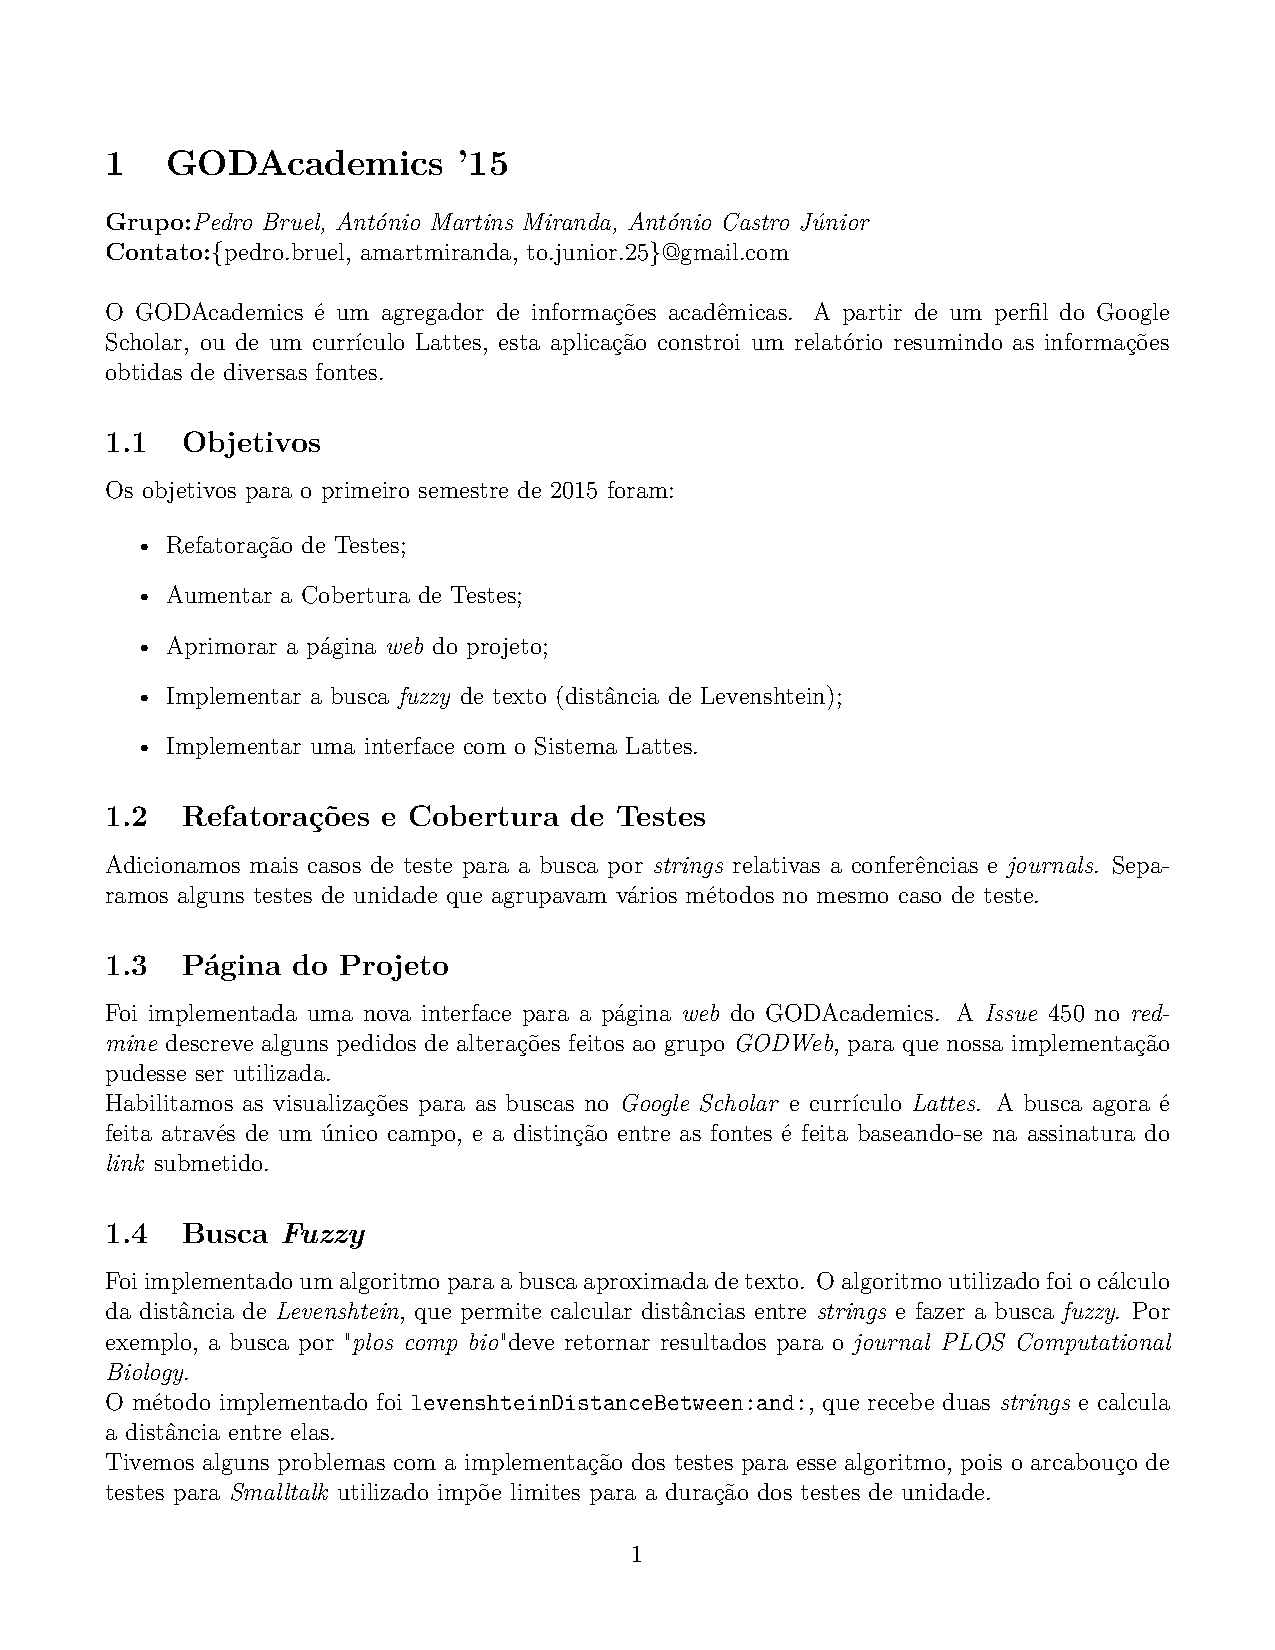
\includegraphics[width=1.3\textwidth, height=1\textwidth, angle =-90 ]{GODAcad}
\end{figure}

\end{document}
